\chapter{Expression in normal human tissues across RNA-Seq studies}
\label{ch:Transcriptomics}

In the perspective of paving the way towards
a generalised baseline expression reference for the normal human,
in this chapter, I assess the similarity
of the tissues sourced from different \Rnaseq\ studies and
the general profiles of their expressed genes.

All the work presented in this chapter was performed by myself under the
supervision of \alvis.
I received invaluable advise and help from my discussions with \nuno.
I also received general feedback and comments from \mar, \johan, \sarah, \gos\
and \wolfgang.

When I started this project in 2013,
little was then known on either the robustness or
the shortcomings and pitfalls of \Rnaseq\ and
its related processing.
Since then, several studies were published assessing \Rnaseq\footnote{See
\Cref{sec:TranssCoop}: \nameref{sec:TranssCoop}}.
A few present a closely related scope to my own investigations, thus
whenever relevant,
I introduce and discuss my results in relation to the published ones.

\TK{Add summary of the chapter.}

\derivativeWork{}
\begin{itemize}[topsep=0pt,nosep]
    \item \fullcite{EBIgxa}
    \item (poster) ECCB 2014 --- A feasibility study:
        Integration of independent RNAseq datasets
    \item (invited talk) GM$^2$ 2013 --- Baseline Gene expression Atlas
    \item (flash talk) CSAMA 2013 --- How quantitative is RNA-seq?
\end{itemize}
\clearpage

In the past years,
\Rnaseq\ rapidly gained popularity
for gene expression studies
due to a larger dynamic range than previous technologies
and the promise to enable quantitative profiling\footnote{%
Prior high-throughput technology microarray assays are very prone
to batch effects and are semiquantitative \mycite{lee:2006}.
}.
However, \Rnaseq\ studies had shown variation in their conclusions. \mycite{seqcmaqc}
At that time,
it appeared that
\Rnaseq\ may share at least partially the problems encountered
with microarray assays.
In fact, \emph{batch effects} restrain the use of direct approaches
for the comparison of independent microarray data
as the resulting insights are poor.\TK{add references}

\section{Working sets}

While many approaches exist,
I usually consider the most conservative routes
\ie\ I rather exclude part of the data to infer conclusions than
keep wider datasets and more partial, biased or ambiguous results.
Thus, I identified the identical core of
explored tissues and expressed genes across the studies.
From this base, I created more robust working sets for my meta-analyses.

Through this chapter, I use two working sets:
\begin{itemize}[topsep=0pt,nosep]
    \item \setOne: 4 tissues --- 12,268 genes across the 5 \Rnaseq\ studies, and
    \item \setTwo: 23 tissues --- 17,551 genes across 2 of these studies.
\end{itemize}

The following \cref{subsec:transtissueOverlap,subsec:transGeneOverlap}
illustrate the construction of these sets.

\subsection{Tissue overlaps across the available normal human RNA-Seq studies}%
\label{subsec:transtissueOverlap}

\Cref{fig:VennStudiesT} presents the tissue overlap between the five datasets.
All datasets share at least four tissues:
\heart, \kidney, \liver\ and \testis.
This 4-tissue set is the base of one working set.

The greatest number of shared tissues is
between the two most recent studies:
\uhlen\ and \gtex.
They constitute the base of a second 23-tissue working set.
This set includes
\Adipose, \Adrenal, \Bladder, \Cortex, \hcolon, \Esophagus,
\Fallopian, \heart, \kidney, \liver, \lung, \Ovary, \Pancreas, \Prostate,
\salivary, \skeletal, \skin, \intestine, \spleen, \stomach, \testis,
\thyroid\ and \uterus.

\begin{figure}[!htbp]
\includegraphics[scale=0.45]{transcriptomics/TransVennTissue.pdf}\centering
\caption[Distribution of unique and shared tissues between the
transcriptomic datasets]
{\label{fig:VennStudiesT}\textbf{Distribution of unique and shared tissues
between the transcriptomic datasets.} The five datasets share four
common tissues: \heart, \kidney, \liver\ and \testis.
The most prominent overlap of tissues (23) is between \uhlen\ and \gtex.
These two sets of tissues are the primary focus of the transcriptomic part of the
study.}
\end{figure}

\subsection{Common measured genes for each of the common tissues sets}%
\label{subsec:transGeneOverlap}
As shown in \Cref{tab:Trans5DF},
many of the transcriptomic datasets I use have been produced through
polyA-selected library protocols.
Hence,
to avoid unnecessary biases\footnote{See
\Cref{subsec:protcodingOnly}: \nameref{subsec:protcodingOnly}.}
I have limited most of my analyses to genes with an annotated biotype as
\emph{\pc} (in \ens{76}),
\ie\ I specially filtered out all the other genes even if they were observed.

\begin{figure}[!hptb]
    \includegraphics[scale=0.46]{transcriptomics/PcodingGenesExpressed1_4tissues.pdf}\centering
    \caption[Unique and shared \pcgs\ expressed
    in the 4 common tissues (≥1 \FPKM)]{\label{fig:ExpGenePcoding1}\textbf{Unique
    and shared \pcgs\ expressed ≥ 1 \FPKM\ in the four common tissues
    across the five studies.}}
\end{figure}

\begin{figure}[!hptb]
    \includegraphics[scale=0.43]{transcriptomics/vennTissue23_1protcodgenes.pdf}\centering
    \caption[Unique and shared \pcgs\ expressed
    in the 23 common tissues (≥1 \FPKM)]%
    {\label{fig:ExpGenePcoding1_t23}\textbf{Unique
    and shared \pcgs\ expressed ≥ 1 FPKM in the twenty-three common tissues
    of \uhlen\ and \gtex\ studies.}}
\end{figure}

The Venn diagram presented in \Cref{fig:ExpGenePcoding1} only includes protein
genes that are observed\footnote{See
\Cref{sec:ExpressedOrNot}: \nameref{sec:ExpressedOrNot}.}
at least once at 1 \FPKM\ for one of the four shared tissues.
The bulk of expressed genes at this threshold is common
to all five datasets.
While each study presents a tiny portion of genes
that are unique,
overall most genes are detected in at least two studies.
The most considerable contingent of shared gene expression is observed
between \uhlen\ and \gtex.

\Cref{fig:ExpGenePcoding1_t23} presents a similar Venn diagram
while focusing on the twenty-three shared tissue set
between \uhlen\ and \gtex\ studies.
The unique genes to each study are negligible compared to the bulk.
They represent less than 0.03\% of the measured genes in each of the studies
(0.026\% for \uhlen; 0.016\% for \gtex).
\begin{comment}
    Gtex:   462/17551 hence 0.02632329\%
    Uhlen:  281/17551 hence 0.01601048\%
\end{comment}

I analysed all the other subgroups of genes
(\ie\ unique to each study or shared only between two to four datasets)
for any functional annotation enrichment.
Neither the \gls{gsea} or the \gls{goa} provided any concluant result.

\section{Prevalence of biological signal over technical variabilities at
tissue level}
\label{sec:Trans_ReproExpresTissue}

As I show in \Cref{ch:expression},
the expression levels of identical tissue samples are highly correlated
within the same study
and allow to group the samples based on their biological source.
Thus, clustering samples across studies offers a quick assessment of
the underlying driving forces for the observed gene expression levels.
A clustering by study means that the technical variabilities are stronger
than any biological expression signature (which is common to microarray studies
\TK{add ref}).
On the other hand,
an interstudy sample clustering by tissue implies that \Rnaseq\ measurements
demonstrate a good (biological) signal over (technical) noise ratio.
In other words,
and as shown on the following heatmaps \Cref{fig:noMitoNoRep4T,fig:noMitoNoRep23T},
\Rnaseq\ is less prone to batch effects and more robust than
microarray assays~\mycite{Taminau2014-hr,Walsh2015-nf}.

\Cref{fig:noMitoNoRep4T} and \Cref{fig:noMitoNoRep23T}
are the respective heatmaps of the hierarchical clustering
of the \treps{}\footnote{\glsxtrlong{TREP}. See \Cref{subsec:averagedTissue}:
\nameref{subsec:averagedTissue}.}
for the four shared tissues across the five datasets and the
twenty-three shared tissues between \uhlen\ and \gtex\ studies.
The heatmaps are based on clustering (Ward's method linkage)
the \treps\ Pearson correlation coefficients
(\pcgs\ expressed at least at 1 \FPKM\
and with the exclusion of mitochondrial genes).

In \Cref{fig:noMitoNoRep4T},
each cluster concurs to a tissue.
The clustering highlights a greater biological similarity of the \treps\
due to their sampling origins than any possible
technical similarity due to library preparation or processing variations.
We may object that
the very different gene expression (and levels) in
\Heart, \Kidney, \Liver\ and \Testis\
\mycite{ramskoldan:2009,Danielsson2015-cn,Sudmant2015-zt,GTExTranscript,Uhlen2015}
may drive this untypical result
and other (less differentiated) tissues may exhibit mitigated ones.
\Cref{fig:noMitoNoRep23T} confirms that the biological origin of the tissues
is the dominant criterion for the clustering of the \treps.
Even if there are a few mixture of \treps,
the majority of them cluster by tissue.
Moreover, in many cases, the mixture occurs for close biologically related tissues,
\eg\ \fallopian\ and \Ovary. Or also, \salivary\
with \Esophagus\ and \Stomach\ \treps.
\Cref{fig:noMitoRep4T} and \Cref{fig:noMitoRep23T}
present heatmaps for the same tissues and studies,
but where every available sample is included\footnote{I.e.\
A few tissues in some studies have more than one sample.
These are either biological or technical (or both) replicates.}
(see also \Crefu{sec:rnaseq-data} and \Crefu{tab:repCorr}).
These two supplementary figures also support that
the biological signal is overly stronger than the technical variations.

\begin{figure}[!htpb]
    \includegraphics[scale=0.84]{transcriptomics/heatmap4TnoMitonoRep_1.pdf}\centering
    \caption[Heatmap of the 4 common tissues across the 5 studies]%
    {\label{fig:noMitoNoRep4T}\textbf{Heatmap of the four common tissues
    across the five studies.}\\All \pcgs\ (except the mitochondrial
    ones) at least expressed at 1 \FPKM\ are included.\\All the
    different \treps\ cluster by tissue of origin
    (instead for example by studies).}
\end{figure}

\begin{figure}[!htpb]
    \includegraphics[scale=0.84]{transcriptomics/heatmap23TnoMitonoRep_1.pdf}\centering
    \caption[Heatmap of 23 common tissues between Uhlén and GTEx studies]%
    {\label{fig:noMitoNoRep23T}%
    \textbf{Heatmap of twenty-three common tissues between Uhlén and GTEx studies.}
    All \pcgs\ (≥ 1 FPKM with the exclusion of the mitochondrial
    genes) are included.\\Most \treps\ cluster by tissues except for a few exceptions:
    There is a mixture of the \tissue{Fallopian tube}
    and \tissue{Ovary} \treps.
    In addition, \tissue{Salivary gland} \treps\ is more correlated to
    \tissue{Esophagus} or \tissue{Stomach} regarding the original study.
    \tissue{Bladder} \treps\ seem to cluster randomly with the others.
    However, these \treps\ are in singleton groups.}
\end{figure}

\Cref{fig:SamedistribPearsCorr} shows the distribution of the Pearson correlation
coefficients for the pairs of identical tissue \treps\
sourced from the different studies
for both of the working datasets \setOne\ and \setTwo.
Most of the Pearson correlations are above 0.5\footnote{Indeed,
there are two exceptions: the
correlation between the \Testis\ \treps\ of \castle\ and \vt\ (0.42)
for the 4-tissues working set and
\Salivary\ \treps\ of \uhlen\ and \gtex\ (0.2)
for the 23-tissues working set.}
even with the lack of any batch effect correction.
The median correlation for the four common tissues across the five datasets is
about 0.7 and 0.84 for the twenty-three tissues between \uhlen\ and \gtex\ studies.
As I mentioned in \Cref{ch:expression},
Pearson correlations are easier to understand, interpret
and then be use as predictors
while Spearman correlations are more robust and thus better fitted for interstudy
comparisons.
See \Crefu{subsec:PearsonVsSpearman}.
Results are even better with Spearman Correlation:
the averages are respectively 0.49 for the 4-tissues sets
and 0.9 for the 23-tissues set and
the median correlations are 0.88 and 0.93.

Both the Pearson\footnote{Despite one major outlier in the second
working set (\tissue{Salivary gland} --- Pearson correlation: 0.2)} and the
Spearman correlation coefficients for the more exhaustive 23-tissues working set
\setTwo\
comprising the two most recent studies,
are higher than the observed correlation for the 4-tissues working set.
Three main reasons may explain this situation:
\begin{itemize}[topsep=0pt,nosep]
    \item In addition of using paired-end sequencing,
        the library preparation protocols were better established
        for these two studies;
    \item The instrument used for the sequencing were
        from the same series (HiSeq 2000 and HiSeq 2500); and
    \item These studies present a higher number of replicates per tissue.
\end{itemize}

\begin{figure}[!htpb]
    \includegraphics[scale=0.65]%
{transcriptomics/TransPearsonDistributionIdenticalOnly.pdf}\centering
\caption[Distribution of the correlation of same tissue pairs for the 4 and 23
tissues working sets.]{\label{fig:SamedistribPearsCorr}\textbf{Distribution
of the Pearson correlation of same tissues pairs for the four and
the twenty-three tissues working sets.}
In general, the Pearson correlations are high when we are
\emph{directly} comparing \treps\ from different studies.\\
The same-tissue pairs in 23-tissues working set (\setTwo) present
a higher median correlation ($0.85$)
and narrower distribution than
in the 4-tissues working set (\setOne) (median$ = 0.74$).
However, \setTwo\ displays one outlier with
a very low Pearson correlation ($0.2$: \salivary\ tissue.).
Sampling, processing issues or biological reasons
may just as well explain this outlier.}
\end{figure}

\Cref{fig:distribCorr} presents the different pairs of tissues across the
datasets in addition to the same tissue pairs.
The pairs comprising different tissues are very lowly correlated in general.

\NB\ In few cases of the 23-tissues working set,
high correlations are also observed for different-tissues pairs
(\eg\ \Fallopian\ and \Uterus\ from \gtex\ study)
(see also \Cref{fig:noMitoNoRep23T}).
It is rather hard to decipher if this may be due to a technical issue
(\eg\ at the collection or library preparation stage)
or because these tissues are biologically very close.

\section{Possible driving force of the closer intratissue rather intrastudy
similarity}

Since \Rnaseq\ allows distinguishing the shared biological origin
of most \treps\ across different studies,
the question then arises as to what is driving these strong interstudy
correlations.

As discussed in \Cref{ch:expression}\footnote{See \Cref{sec:ExpressedOrNot}:
\nameref{sec:ExpressedOrNot}},
correlation coefficients measure the dependence between (here) two tissue \treps\
and are subject to outliers and the skewness of the distributions.
As I have excluded the \emph{undefined}\footnote{I.e.\
\emph{unobserved} --- See also
\Cref{subsec:ExpressedOrNot-undefined}: \nameref{subsec:ExpressedOrNot-undefined}}
genes from the analyses,
the high correlations have another rationale than spurious null values.
Thus, the next intuitive step is to test
whether a particular subset of the genes may drive the correlation coefficients,
\ie\ are the highest, the most variable or another group of genes
the underlying reasons of the strong correlations.

\subsection{Highest expressed genes}

The notion of highest expressed genes may be trivial,
but it is worth remembering that the normalisation methods are impacting
the final expression values.
As presented in \Cref{ch:background} all \Rnaseq\ values are inherently relative
to the observed genes and the assumptions underlying the normalisation.
Thus, from the same unnormalised (\ie\ \emph{raw count}) processed sample,
depending on the normalisation method
(see \Cref{subsub:norm}:~\nameref{subsub:norm}),
the gene expression values and their final ranked order may be very different.
In the present case though,
I avoid many biases
by processing the data with consistent methods and annotation
and by excluding selected sets of
genes\footnote{See \Cref{sec:bias_sources}:~\nameref{sec:bias_sources}}.
Concomitantly, if I had picked another normalisation method than \FPKM\footnote{See
\Cref{eq:rpkm-fx}},
the exclusion filters applied to create \setOne\ and \setTwo\ would impact
a different set of genes.

To test the influence of highest expressed genes on correlation coefficients,
I chose to visualise the trend of the correlation
as a function of expression value thresholds.
For \Cref{fig:CorHighExp4T} and \Cref{fig:CorHighExp23T},
I computed the correlations of genes expressed above a cut-off
for each pair of identical tissues within each of the two working datasets.
The cut-off is a range of possible (integer number) value of gene expression
(using 10 as a step).

%\begin{sidewaysfigure}[!htpb]
\begin{figure}[!htpb]
    \centering
    \begin{subfigure}[b]{0.4\textwidth}\centering
        \includegraphics%[height=0.4\textheight]
        {transcriptomics/HeartEvolHighExp4P-1.pdf}
        \caption{Heart}\label{fig:CorHighExpHeart4T}
    \end{subfigure}%
~%
    \begin{subfigure}[b]{0.4\textwidth}\centering
        \includegraphics%[height=0.4\textheight]
        {transcriptomics/KidneyEvolHighExp4P-1.pdf}
        \caption{Kidney}\label{fig:CorHighExpKidney4T}
    \end{subfigure}

    \begin{subfigure}[b]{0.4\textwidth}\centering
        \includegraphics%[height=0.4\textheight]
        [scale=0.4]{transcriptomics/LiverEvolHighExp4P-1.pdf}
        \caption{Liver}\label{fig:CorHighExpLiver4T}
    \end{subfigure}%
~%
    \begin{subfigure}[b]{0.4\textwidth}\centering
        \includegraphics%[height=0.4\textheight]
        [scale=0.4]{transcriptomics/TestisEvolHighExp4P-1.pdf}
        \caption{Testis}\label{fig:CorHighExpTestis4T}
    \end{subfigure}
    \caption[Pearson correlation coefficient evolution based on the expression
    levels of the genes considered for each of the 4 common tissues]{%
\label{fig:CorHighExp4T}\textbf{Pearson correlation coefficient evolution
    based on the expression levels of the genes considered for each of the four
    common tissues across the five studies.}}
\end{figure}
%\end{sidewaysfigure}

For the 4-tissues working set \setOne\ (\Cref{fig:CorHighExp4T}),
except for very few pairs, the highest correlations correspond to
the lowest cut-off of 1 \FPKM\@.
In fact, the same tissue \trep\ correlation coefficients
are increasing as the expression cut-off is lowered
(the calculations involve then more genes).
Here below, the few exceptions grouped by tissue:
\begin{eqlist}[\eqliststarinit\def\makelabel#1{\bfseries#1}\labelsep1em]
\item[Heart] \uhlen{}-\gtex\ pair
\item[Kidney] \uhlen{}-\gtex, \castle{}-\uhlen\ and \castle{}-\gtex\ pairs,
\item[Liver]  \vt{}-\ibm, \ibm{}-\uhlen\ and \ibm{}-\uhlen\ pairs;
\item[Testis] \ibm{}-\uhlen, \vt{}-\gtex, \vt{}-\uhlen\ and \uhlen{}-\gtex\ pairs
\end{eqlist}

In the context of the 23-tissues working set (\Cref{fig:CorHighExp23T}),
many more tissue pairs present very high correlation for subsets of their highly
expressed genes, \ie\ \skeletal, \Thyroid, \Cortex, \Uterus, \Kidney.
Unfortunately, these specific examples are insufficient
to derive any consensual threshold for future work.
Moreover,
for any similar tissue pair of \setTwo,
considering every \pcg\ expressed at least at 1 \FPKM\ is usually
far better than selecting any highly expressed genes subset
(except for \kidney).

\begin{figure}[!htpb]
    \includegraphics[scale=0.8]{transcriptomics/T23EvolHighExp23P-1.pdf}\centering
    \caption[Pearson correlation coefficient trend based on the expression
    levels of the genes considered for each of the 23 common tissues]{%
\label{fig:CorHighExp23T}\textbf{Pearson correlation coefficient trend based
on the expression levels of the genes considered
for each of the twenty-three common tissues between \uhlen\ and \gtex.}
Almost only the complete set of common expressed \pcgs\ of each tissue gives
the highest correlations.}
\end{figure}

The highest cut-offs present many anticorrelations.
These are mathematical artefacts.
They involve very few genes
and as such the correlations are more sensitive to any change
(see \Cref{sec:whyAnticor}).

As the interstudy Spearman correlations of same tissue pairs
are higher than the Pearson ones,
I have tried to ponder for the possible difference in the expression magnitude
across the studies\footnote{Due to particular batch effects in each study}
while the highest expressed \pc\ may have similar ranks
for a given tissue.
Thus, I have explored the ratio of the common most top expressed
genes across the studies to the number of genes considered
(see \Cref{sec:overlapHighExp}).
The general trend of the overlap ratio follows a random one.
Indeed, only the top highest \pcgs\ in each tissue
present high overlap ratios between the studies.
All the other \pcg\ ranks are indistinguishable from any random ordering.

\begin{comment}
While a study of the highly expressed \pcgs\ is interesting,
its ability on explaining the underlying reasons
of the strong interstudy tissue correlations seems limited at best
or even inadequate.
\end{comment}

Together, these results indicate
that the highest expressed genes are unable to explain
the intratissue/interstudy high correlations.
Thus, I have considered other candidates
such as the most variable genes.


\subsection{Most variable genes}
As correlations translate the relationship strength,
similar gene expression variation patterns for the tissues
across the independent studies can also explain the strong correlations.
Moreover, other things being equal,
Pearson correlations are higher
when the observations are more (rather than less) variable.
This effect is often referred as
\emph{restricted range}.~\mycite{CorrelationImpactingFactors}

There are several available estimators to describe the gene expression variability
\eg\ the standard deviation~(sd) the variance~($sd^2$) or the coefficient of
variation~($\frac{sd}{mean}$).
I only report here the results based on the coefficients of variation.

The \gls{cv} allows assessing
the dispersion of the gene expression values
across the tissues within each dataset.
As it contextualises the values to the mean,
it is a more straightforward estimator to interpret than
the standard variance itself,
in particular for interstudy comparisons.

\begin{comment}
Visualising the \gls{cv} distribution of
gene expression for the working set \setOne\ (see \Cref{fig:HistCV4T})
allows determining whether they are similar across the five transcriptomic studies
or that inferring conclusions requires more cautions.
\end{comment}
As depicted in \Cref{fig:HistCV4T},
the distribution of gene expression \cvs\ presents a similar pattern
across the five studies of \setOne,
it suggests that extra steps to infer conclusions are non-compulsory here.

\begin{figure}[!htpb]
    \captionsetup{singlelinecheck=off}
    \includegraphics[scale=0.75]{transcriptomics/distributionCV_4commonTissues.pdf}%
    \centering
    \caption[Coefficients of variation across the 5 studies for the set of common
expressed genes and tissues]{\label{fig:HistCV4T}\textbf{Distribution of the
\cvs\ (cv) across \setOne: common set of expressed \pcgs\
across the four common tissues:
\{\Heart, \Kidney, \Liver, \Testis\}
across the five studies.}\\
The coefficients of variation (\gls{cv}) of the \pcgs\ (12,268) of the four tissues
present the same bimodal distribution profile across the five studies.
\\These profiles present two peaks: at $0.5$ and $2$.\\
After more investigation, it appears that
the genes with a \gls{cv} lesser than or equal to $0.5$ have
a similar expression profile to a left-truncated version of
the complete gene set ones (due to the $1$ \FPKM\ cut-off)
as in \Cref{fig:distribPlot}.
On the other hand, the \pcgs\ with a coefficient of variation
equal to or greater than $1.5$ have two kinds of distinct profiles:
{\small
\begin{itemize}[topsep=0pt,nosep,leftmargin=95pt,listparindent=5pt]
    \item The gene expression is low across the four tissues and
        it is above the cut-off of $1$ \FPKM\ only once; or
    \item The gene expression is specifically high for one single tissue
        in regard to the three others.
\end{itemize}
}}
\end{figure}

The five datasets present a two peaks.
One at 0.5 which characterises genes
that are quite invariant in their expression across the four tissues within each
dataset.
Another subset of genes form a peak for \cv\ equals 2.
These last group of genes are the most variable ones in each datasets.
While there is some overlap of the most variable genes
between the five datasets,
it is only partial (see further \Cref{fig:cvEvol5DF}).

A simple approach to test if the commonly most variable genes
are the driving force of the correlation is
to study the difference of their correlation with
the remaining set of considered \pcgs.
If the most variable \pcgs\ are driving the correlation
then their group has to present higher correlations than the second set.

After ranking the \pcgs\ in decreasing order of their \cv\ within each study,
I select the intersection of genes in the first quarter across them
to create the set of most variable genes $S_{most~Variable}$.
The remaining genes are constituting the second group $S_{remaining}$\footnote{%
$S_{remaining} = $ \setOne{}$- S_{most~Variable}$}.
For both of these gene groups, $S_{most~Variable}$ and $S_{remaining}$,
I calculate the coefficients of correlation for all possible tissue couples.

\begin{figure}[!htpb]
    \includegraphics[scale=0.70]%
    {transcriptomics/TransPearsonDistributionIdenticalDifferentHighestCVgenes.pdf}%
    \centering
    \caption[Comparison between the most variable genes with all the other ones]%
    {\label{fig:test_mostvaribleVSevery}\textbf{Comparison between
    the most variable \pcgs\ with the remaining genes in \setOne\ set.}
    For both the most variable group $S_{most~Variable}$
    and the remaining one ($S_{remaining}$) of \pcgs,
    the correlations between identical interstudy tissues are greater
    than any correlation between different (even intrastudy) tissues.
    The distribution of the intertissue correlations for $S_{most~Variable}$
    show that these genes are showing a tissue signature
    while they are lacking an interstudy linear relationship for same tissue
    couples.}
\end{figure}

\Cref{fig:test_mostvaribleVSevery} summarises this analysis.
It shows the Pearson correlation distribution
for these two groups of \pcgs\ in \setOne.
One-sided \Welchttest\footnote{See \Cref{mini:ttest}.}
allows rejecting the null hypothesis $H_0$ at 95\% of confidence.
The mean of the %(Pearson and Spearman)
correlation coefficients
calculated with the common most variable \pcgs\ are significantly greater than
the ones calculated with the remaining set of \setOne genes\footnote{Though,
a two-sided \Welchttest\ compels to accept the $H_0$ hypothesis:\\
the two populations of coefficients correlation are not significantly different
(\pvalue{= 0.06594}).}.

For Pearson correlation:
$mean_{most~Variable}=0.76$ and $mean_{remaining}=0.68$
(\pvalue{= 0.03295}).
Thus, the common \pcgs\ with the highest \cv\
discriminate better between the identical and different tissues.

However, for both groups,
$S_{most~Variable}$ and $S_{remaining}$,
the \treps\ across the studies cluster mostly by tissue rather than
original study.
See and compare \Cref{fig:heatmapMost25pVariable,fig:ReverseheatmapMost25pVariable}.
These supplementary figures respectively present
the heatmaps (with clusterings) of the tissues
based on their Spearman correlation for the most variable (\cv) \pcgs\
and all other remaining genes of \setOne.
The \treps\ cluster mainly by their original tissue.
In fact, the only exception is that
\castle\ tissues cluster primarily by study
once I exclude the most variable genes.

\begin{figure}[!htpb]
    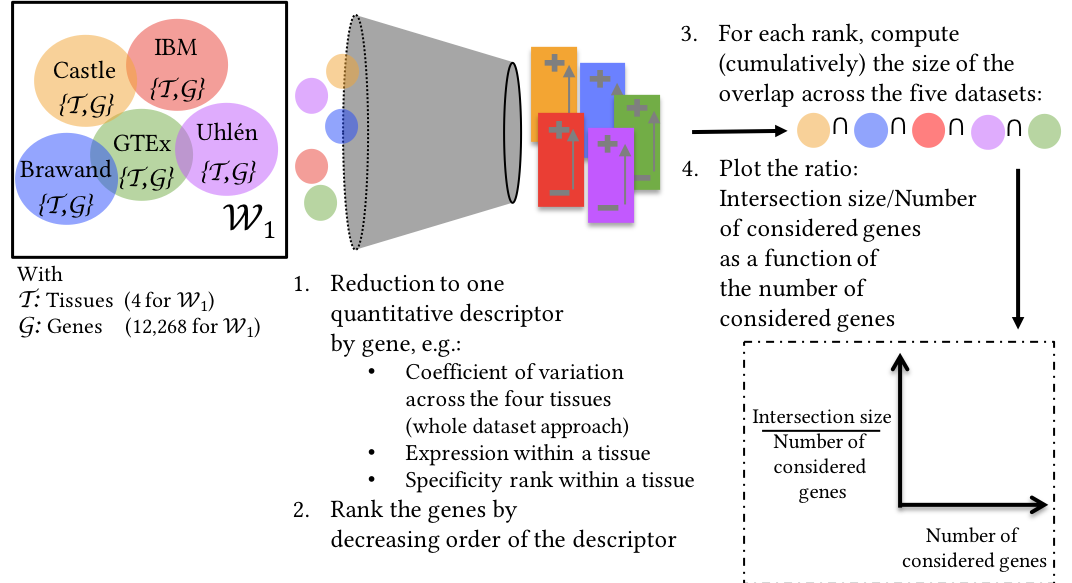
\includegraphics[scale=0.9]{transcriptomics/ConceptOverlap.png}\centering
    \caption[Overview for the comparison of the genes across the five
    studies based on a ranked descriptor 5 studies]{\label{fig:overlapConcept}%
    \textbf{Overview for the comparison of the genes across the five
    studies based on a ranked descriptor.}
    The first step applies individually to each of the studies
    within the working dataset (\ie\ here \setOne).
    It consists in extracting a single value per gene
    (\eg\ a statistic or any other quantitative descriptor)
    either for the entire \emph{d}ataset (referred thereafter as \emph{D-approach}) or
    for each \emph{t}issue in each dataset (referred as \emph{T-approach}).
    The next steps include
    computing (cumulatively) the intersection size number for each rank
    and plotting this number divided by the rank
    in function of the number of considered genes (\ie\ rank).}
\end{figure}

\begin{figure}[!htpb]
    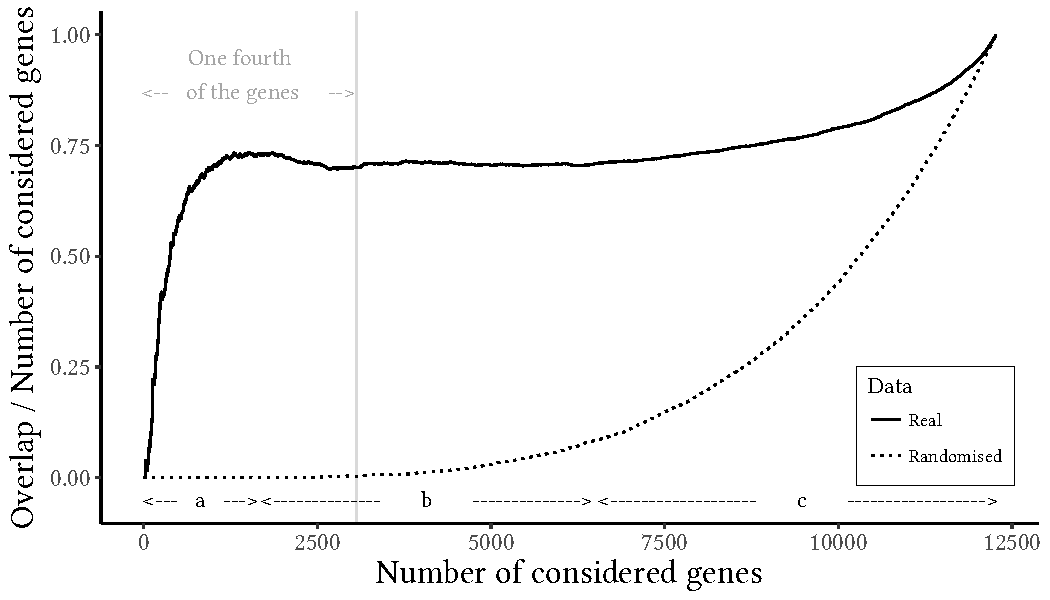
\includegraphics[scale=0.9]{transcriptomics/CVevolCumul5DF_line-abc.pdf}\centering
    \caption[Intersection size of \setOne\ genes (ranked by cv)]%
    {\label{fig:cvEvol5DF}\textbf{Intersection size course
    of \setOne\ genes (based on their coefficient of variation rank
    in each of the five studies).}
    There are three main parts.
    There is an initial strong growth (a)
    %followed by a short plateau (b)
    %before a slight decrease (c)
    which then settles a plateau (b).
    Eventually, the ratio increases slowly again
    until reaching the expected ratio of $1$ once all the genes from \setOne\
    are included (c).
    The first quarter of the genes covers (a) and a part of (b).
    Apart from (a),
    the overlap of shared genes between the five datasets when ranked on their
    coefficient of variation is above 70\%.
    The sigmoid curve (dashed line) is based on randomised data
    where permutations break the original order of the genes. (All the gene
    expressions levels within each dataset are permuted while the pattern of
    expression across the tissues is conserved. This operation is performed 10,000 times.
    The dashed line is a summary of all these permutations).
    There is a significant dissimilarity between the real and the randomised data.}
\end{figure}

To avoid any oversight due to the arbitrarily chosen number (first quarter)
of the most variable genes,
I have also studied the course of the intersection size of the common genes
across the five studies
in function of the number of \setOne\ genes that I consider.
\Cref{fig:overlapConcept} illustrates my general approach.
After ordering the genes by decreasing order of their \cv\
within each of the datasets comprised in \setOne,
I have calculated the size of overlap for each rank (\ie\ from 1 to 12,268)
between the five datasets.
To help with the interpretation,
I finally divide the previous figure by the rank.

\Cref{fig:cvEvol5DF} presents the result.
Many of the most variable genes are commonly present in the top tier of the
five studies, though they have different individual rank.
Indeed, there is a strong growth for about the first 1,250 genes that then
settles a plateau which increases toward the final ratio ($1$).
Using the first quarter of the most variables genes as a cut-off appears
to be an acceptable threshold
as it comprises the primal growth and part of the plateau.

\begin{comment}
If the previous analysis was to include
only the first 1,250 most variable genes
the results of \Cref{fig:heatmapMost25pVariable} may be even greater.
However, the dissimilarities highlighted by \Cref{fig:ReverseheatmapMost25pVariable}
would also be greater.
\end{comment}

In conclusion, while the most variable genes have a significant influence
on the strong and biologically meaningful correlations,
there must be other gene categories contributing.

\begin{comment}
The most variable genes present overall a distinct expression pattern
where one tissue stands out with a much higher expression.
Moreover, these patterns are mostly consistent across the independent studies
(see \Cref{fig:expressionMostvariableG}).
\end{comment}

\NB\ One main drawback when considering the most variable genes is
the descriptor summarises the genes across all the tissues.
So,
the results may significantly vary
depending of the composition of the working set
and this analysis ought to be rerun.

\subsubsection{Detecting variable genes by tissue with Hampel's test}\label{subsub:Hampel}


The Hampel's test is robust for detecting outliers~\mycite{Davies1993-nv,Pearson2002-im}
in data that are identically and independently distributed (i.i.d.)~\mycite{Liu2004-kf},
while easy to implement and use~\mycite{LinsingerHampel}.
Many interstudy researches in the literature use Hampel's tests,
\eg~\mycite{LinsingerHampel,Lewczuk2006-wq,Rocke1983-qa,Apfalter1999-ca}.

After implementing the method (see \cref{algo:hampel}),
I have applied it on the whole original datasets, \setOne\ and \setTwo.


Genes that undeniably have an expression profile
that varies in function of the tissue,
%and thus impact positively the correlations,
are the tissue specific genes.

\begin{figure}[!htpb]
    \includegraphics[scale=1]{transcriptomics/hampel5DF4Tissues.pdf}\centering
    \caption[Expression of the genes picked with Hampel method]{\label{fig:hampelExp}%
    \textbf{Expression of the genes picked consistently with the Hampel method
    in each study solely in one tissue.}}
\end{figure}

\subsection{Tissue specific genes}\label{sub:TisSpeGene}

Another good candidate to drive higher correlations
between identical interstudy \treps\ than intrastudy ones are
the tissue specific genes.

There are different definitions in the literature.
There are also database as \eg\ \gls{TIGER}.

As a matter of fact, the expression patterns of many of
the most variable genes across the different tissues
are globally uniform aside one or two tissues
where the expression is higher (see \Cref{fig:expressionMostvariableG}).

\subsubsection{Use of prior knowledge: TiGER database}\label{subsub:Tiger}

\gls{TIGER} is a database that reports tissue-specific genes for thirty tissues
(based \glspl{EST} experiments).

After retrieving the list of genes from the thirty types of reported tissue, I have mapped the Refseq ID to Ensembl gene ID (Ensembl 73).
I filtered out all the genes reported more than one tissue. The following heatmap (Figure 7) shows a sample of these tissue specific genes reported by TIGER. We can observe different subsets of genes: the ones which are confirmed, the ones that are infirmed (i.e. expressed everywhere) and the ones that are attributed to another tissue.


One database in particular, \gls{TIGER},
has collate tissues-specific genes (based \glspl{EST} experiments)
for thirty independent tissues\footnote{See \Cref{sec:supplTiger}: \nameref{sec:supplTiger}
for the complete list.}
After I retrieved all thirty lists,
I have translated the gene lists from \gls{Refseq} to \gls{Ensembl} (\hg{38},v. 76).
Then, I removed all duplicates due to the translation and I also filtered out
all the genes identifiers that I found in more than one tissue.
Thus, for each tissue,
I have a list of identifiers that are specific to that tissue only.




\subsubsection{Fold change method}\label{subsub:TisSpeGeneMethodPerso}

\begin{figure}[!htpb]
    \includegraphics[scale=1]{transcriptomics/mostSpe4TP.pdf}\centering
    \caption[Cumulative shared set of genes sorted by their specificity in each
    tissue across the 5 datasets]{\label{fig:mostSpe4T}\textbf{Cumulative shared
    set of genes sorted by their decreasing order of specificity in each tissue
    across the five datasets.} Results are better than for the highest expressed or
    the most variable genes.}
\end{figure}

Thus, the tissue specific genes are also contributing to provide a stronger
biological signal over the technological noise.

\subsection{Uhlén categories}\label{sub:UhlenGeneCat}

Finally, best may be to use different categories to describe the data as have
done Uhlén and co for example. Ca change de répartir les gènes que en exprimé/pas exprimé
et en niveau d'expression.

They change the definition of their categorisation
between their two related papers~\mycite{Uhlen2014} and~\mycite{Uhlen2015}.
The definition I am using is a based on their second paper,
but with some subdivisions they presented in the first one.

\pagestyle{plain}
\begin{landscape}
\begin{table}[]
\centering
\caption[Uhlén et al.\ gene categories]{\label{tab:UhlenCategoriesProtCoding}%
\textbf{Uhlén et al.\ gene categories}\\
\footnotesize{Apart the undetected genes and the ones expressed below 1 \FPKM,
a gene may be referenced in several categories.}}

%\begin{tabular}{@{}lllllllllll@{}}
\begin{tabular}{@{}ccccccccccc@{}}
\toprule
\multicolumn{2}{c}{\multirow{2}{*}{\begin{tabular}[c]{@{}c@{}}\ens{76}
    \\($\sim$22,500 protein\\coding genes) \end{tabular}}} &
\multirow{2}{*}{\begin{tabular}[c]{@{}c@{}}\\Not\\detected\end{tabular}} &
\multirow{3}{*}{\begin{tabular}[c]{@{}c@{}}Not expressed\\ at 1 \gls{FPKM}\\
    cut-off\end{tabular}} &
\multicolumn{2}{c}{Mixed expression} &
\multicolumn{2}{c}{Ubiquitous expression} &
\multirow{2}{*}{\begin{tabular}[c]{@{}c@{}}\\Group \\Enhanced\end{tabular}} &
    \multirow{2}{*}{\begin{tabular}[c]{@{}c@{}}\\Tissue\\ Enhanced\end{tabular}} &
        \multirow{2}{*}{\begin{tabular}[c]{@{}c@{}}\\Tissue\\ Enriched\end{tabular}} \\
    \cmidrule(lr){5-8}
\multicolumn{2}{c}{}
    &  &  &
    \begin{tabular}[c]{@{}c@{}}Low\\ (\textless\ 10 \gls{FPKM})\end{tabular} &
        \begin{tabular}[c]{@{}c@{}}High\\ (≥ 10 \gls{FPKM})\end{tabular} &
            \begin{tabular}[c]{@{}c@{}}Low\\ (\textless\ 10 \gls{FPKM})\end{tabular} &
    \begin{tabular}[c]{@{}c@{}}High\\ (≥ 10 FPKM)\end{tabular} &  &  &  \\
        \midrule
        \multicolumn{1}{c}{%
        \multirow{6}{*}{\rotatebox[origin=c]{90}{\parbox[c]{3cm}{\centering Whole
        dataset}}}} &
        Castle & 3,403 & 3,268 & 8,773 & 1,033  &
        1,399  & 634   & 11   & 3,664   & 1,975 \\
        \multicolumn{1}{c}{} & Brawand & 2,964 & 3,095 &
        8,034 & 1,788  & 1,760 & 958   & 0  &
        2,729  & 2,548 \\
        \multicolumn{1}{c}{} & IBM & 2,693 & 2,605  &
        7,325  & 1,406  & 1,135 & 858  & 322 &
        5,248  & 2,453  \\
        \multicolumn{1}{c}{} & Uhlén & 2,662 & 1,747 &
        5,769 & 1,053  & 456 & 406  & 2,511  &
        5,201  & 2,333  \\
        \multicolumn{1}{c}{} & GTEx & 2,197  & 1,886  &
        5,556  & 1,117 & 687  & 698  & 3,859  &
        4,356  & 1,919 \\ \cmidrule(l){2-11}
        \multicolumn{1}{c}{} & Consensus & 2,197 & 486  &
        1,749  & 221  & 33  & 161  & 0  & 677  &
        \begin{tabular}[c]{@{}c@{}}531 $[$518$]$\end{tabular} \\
            %\multicolumn{1}{c}{} & \footnotesize{without Gtex} &
            %\footnotesize{2,413} & \footnotesize{638} & \footnotesize{2,152} &
            %\footnotesize{286} & \footnotesize{63}  & \footnotesize{179} &
            %\footnotesize{0}  & \footnotesize{814} &  \footnotesize{587}  \\
            \midrule
\multirow{6}{*}{\rotatebox[origin=c]{90}{\parbox[c]{3.5cm}{\centering Common\\
4 tissues\\ Working datasets}}} &
Castle & 19,066 & 2,994 & 8,589 & 1,513 &
2,994 & 1094 & --- & --- & 2,185 \\
& Brawand & 19,505  & 2,962  & 8,626  & 2,228
& 2,962  & 1251 & --- & --- & 3,672  \\
& IBM & 19,776  & 2,989 & 8,534 & 1,954 &
2,989  & 1212  & --- & --- & 2,824  \\
& Uhlén & 19,807 & 2,917 & 8,367 & 2,227 &
2,917  & 1190  & --- & --- & 3,730  \\
& GTEx & 20,272 & 3,870 & 8,988  & 2,312 &
3,870  & 1427  & --- & --- & 3,554  \\
\cmidrule(l){2-11}
& Consensus & 1,973 & 550 & 3,351 & 649 &
550  & 439 & --- & --- & 1,412  \\
%& \footnotesize{without Gtex} & \footnotesize{2,413}  & \footnotesize{2,186}  &
%\footnotesize{3538}  & \footnotesize{639}  & \footnotesize{576}  &
%\footnotesize{439}  & \footnotesize{---} & \footnotesize{---} & \footnotesize{1,462}
\midrule
\multirow{3}{*}{\rotatebox[origin=c]{90}{\parbox[c]{1.7cm}{\centering Common\\ 23
tissues\\ Working datasets}}} & Uhlén & 2,662  & 1,970  &
6,160 & 1,135 & 594  & 427 & 1,285 &
5,776 & 2,518 \\
& GTEx & 2,197 & 2,258 & 6,966  & 1,540 &
1,822  & 997 & 1,048 & 5,496  & 2,460 \\
\cmidrule(l){2-11}
& Consensus & 2,197 & 1,544 & 4,936 & 791 &
423 & 417 & 558 & 4,223 & 1,885 \\
\bottomrule
\end{tabular}
\end{table}
\end{landscape}
\pagestyle{scrheadings}


\subsection{Curated sets}\label{subsec:Trans_curatedSets}
Protein coding genes that were characterised consistently
as any of the previous categories across the five datasets
are provided as supplementary data.


\section{Discussion}\label{sec:Trans_discussion}
\TK{when I started no paper, now overloads}: list them and compare to my own
work. Meta-analysis\ldots

Small overlap of tissues: so scientifically not very good.
However, most of the genes expressed everywhere.
But, in general Biology >>> Technical.

Apart Castle but Castle method not really used any more. So it might be because of
the protocol which is harder to set up or not mature (maybe can be improved) or
maybe the method gives different measurements due to what it fishes and
normalisation methods which are not very good for that (biases).

Quite expectedly, as these analyses were incorporating more studies,
the results improved greatly.
Indeed, as I focalise the study on the shared genes across the studies,
I bias the analyses towards the genes with more robust expression profiles
that may be measured with \Rnaseq.



Petit blabla sur la normalisation (de nouveau), normalisation pas adapté
ERCC ptet 1 idée mais pas vraiment un internal standard.


New set of tissue spe.
Hampel method
Quantile normalisation\ldots

MAJ tissues spe de Tiger (ne pas oublier la discussion sur l'annotation)

tend vers une 1 limite mais pas mal de redéfinition

\TK{start speaking about the normalisation a bit, deseq, tpm, \ldots}

Ouverture: là, où au début on avait pas beaucoup de data avec des réplicats
biologiques pour le normal, on a commencé en avoir pas mal. Du coup, \nuno\
a analysé les genes avec un faible coeff de var. On a défini ca comme housekeeping
genes.


\NB\
\begin{comment}
Indeed, the analyses involving the variance instead give
fewer insights.
\end{comment}
Also, it is worth mentioning that the results presented here
improve considerably when analyses include \uhlen\ \etal\ and the \gtex\ studies.
\begin{comment}
Indeed, preliminary results (only based on \castle, \vt\ and \ibm\ studies)
were far worse.
\end{comment}
And unsurprisingly, updating the human genome version from \hg{37} to \hg{38}
for the reconstruction
step\footnote{See \Cref{subsec:reconstruction}: \nameref{subsec:reconstruction}}
also enhances significantly the results.



